% In this chapter, I will describe the techniques used to characterize the BeGe detectors,
% including tests involving e.g. resolution, noise, charge collection, multi-site rejection.
%
% Results of the tests will be presented
%
% It is also possible to present some of my hardware/software development work here
% since this is relevant to the characterization studies.  I imagine these
% generally will occupy appendices.

\chapter{Development of a Digital Data Acquisition System for P-type Point Contact Detectors}
\label{chap:DAQDevel}
	\section{Introduction} 
	
	The detectors in the \MJ~\minmod~will be readout using a digital data acquisition system using fast ADCs to digitize raw preamp traces to be used in later pulse-shape analysis.  The requirements of a digital DAQ system for the \minmod~were investigated, in particular focusing on refining the hardware specifications needed to achieve the physics goals of the project.  These specifications must be sufficient to achieve two general goals: (1) background reduction through pulse-shape analysis, especially in the $\nonubb$ region-of-interest, and (2) low-energy performance enabling both background reduction at $\qval$ and sensitivity to low-energy physics (dark matter).  
	
	 This appendix focuses on investigations of several issues of the DAQ:
		\begin{itemize}
			\item Sampling rate 
			\item Operational stability
			\item Low-energy performance
			\begin{itemize}
				\item Triggering
				\item Low-energy resolution
			\end{itemize}	
		\end{itemize}
but does not detail the development of all the hardware and software to run most of these tests.  For more information regarding some of that work, please see Appendix~\ref{app:ORCASoftwareChapter}.  %Chaper~\ref{chap:DeploymentPPC2Soudan} describes efforts to test elements of the DAQ systems presented here in a deployed, underground environment.

	Because P-type Point Contact detectors will be used in the \MJ~\minmod, it was necessary to use such a detector for some of these tests.  A \ppc~detector (henceforth referred to as \ppc2) was procured by PNNL in January 2008 to be used in studies aimed at more clearly understanding the detector technology~\cite{Orr2007}.  Initial tests took place in the laboratory, focusing on basic operation and pulse-shape analysis techniques relevant for background reduction in the $\nonubb$ region-of-interest and for Dark Matter searches~\cite{Orr2008}.  Some of these results are presented here (see Section~\ref{sec:HeadToHeadCompare}).  Following these tests, in November 2008 the detector was deployed underground at Soudan National Laboratory at a depth of 2100~m.w.e.~to investigate both the low-energy performance and operational stability.
	   
	\section{Baseline DAQ system}

	The baseline system for development used the Gretina Mark IV digitizer
designed by the GRETA collaboration~\cite{Anderson:2009p1293}.  This
VME64x-based ADC digitizes 10 independent channels at 100~Ms/s with a
resolution of 14 bits.  The card was read out using the ORCA DAQ software
developed at the University of Washington and at the University of North
Carolina~\cite{Howe04,Howe08,ORCA}.%, see also
%Appendix~\ref{app:ORCASoftwareChapter}).  
	
	\section{Digitizer comparison tests}
     	\label{sec:HeadToHeadCompare}
     	% Comparison between 100 MS/s and other cards.
	
	Since the Gretina card is being considered as a candidate card for the \MJ~\minmod, head-to-head tests between it and digitizers with different characteristics were necessary.  The purpose of these measurements was to investigate how the specifications of each digitizer affected its ability to perform pulse-shape analysis for background reduction through multi- and single-site event selection.  The decided method was to take data from \ppc2 concurrently with different digitizers using a $^{232}$Th source.  $^{208}$Tl, a daughter in the thorium chain, produces a double-escape peak (DEP) at 1592.5~keV which is predominantly composed of single-site events and is commonly used (e.g.~\cite{Abt2007332,Orrell:2007tt}) to test pulse-shape analysis algorithms.  After taking concurrent data, the waveform data were processed using the same algorithm to determine how each digitizer performed.
	
		\subsection{Measurement}
	     	\label{sec:HeadToHeadCompareMeasurement}     
	The measurement with \ppc2 took place at Pacific Northwest National Laboratory running a round-robin test with 3~different digitizers, two cards at a time.  The digitizers used were the Gretina Mark IV, XIA DGF4-c, and the XIA Pixie-4, details about which are given in Table~\ref{tab:HeadToHeadComparisonDetectorChars}.  The \ppc2 preamp had two identical signal outputs, and so each of these was AC-coupled to one of the two digitizers being used for each test.  The inhibit output, which generated a logic pulse when the reset circuitry of the preamp was active, was split and input in to each digitizer.  The time signature of the inhibit pulse was later used to synchronize the data sets (see Section~\ref{sec:HeadToHeadCompareAnalysis}).  
	
	The DAQ software used for both XIA cards was an IGOR Pro-based package designed and shipped by XIA.  	The setup for the Gretina card was similar but simpler to that described in Section~\ref{sec:DeploymentPPC2SoudanDAQSystem}, again using ORCA to readout the card.  The data from each DAQ system were converted to a common format and stored in ROOT files using MGDO data objects.  More details on MGDO can be found in Appendix~\ref{app:MGDO}.  Each XIA card was run in parallel with the Gretina card and around 2~hours live-time of source data were taken for each pair, though the wall clock time was roughly 2 (4) times this during runs with the DGF4-c (Pixie-4) due to induced the dead-time of the XIA cards.  (The Gretina card is designed to be deadtime-less.)  
		
			\begin{table}
				\centering
				\begin{tabular}{l|c|c|c}
					Name & Sampling Rate & Bit Resolution & Form Factor \\
					\hline
					XIA DGF4-c & 40 Ms/s & 14 bits & CAMAC \\
					\hline
					XIA Pixie-4 &  75 Ms/s & 14 bits & PCI \\
					\hline
					Gretina Mark IV &  100 Ms/s & 14 bits & VME64x \\										
					\hline					
				\end{tabular}
				\caption[Comparison of digitizer characteristics]
				{Comparison of digitizer characteristics used in this test.}
				\label{tab:HeadToHeadComparisonDetectorChars}
			\end{table}	
		
		\subsection{Analysis}
	     	\label{sec:HeadToHeadCompareAnalysis}     		
		 % Synchronizing two systems is the basic idea here, go over how this is actually done
	The data were converted to the ROOT-based MGDO format using the OrcaROOT processing libraries.  The amplitudes of each Gretina pulse were calculated using an offline trapezoidal filter.  The value of the onboard trapezoidal calculation was used for each XIA card.  Once converted, the runs with each pair of cards were synchronized together using the timing of the inhibit pulse.  The basic algorithm searched for common time differences between reset pulse events, accommodating the fact that the XIA cards tended to miss numbers of these events given their dead-time and that their 32-bit on-board clocks rolled over more often than the 48-bit clock on the Gretina card.  Once a catalog of synchronized events was determined, the data were compiled into a single set of ROOT files for later pulse-shape analysis.  An example of a synchronized event is shown in Figure~\ref{fig:HeadToHeadPulseExample}.  The difference in decay time constants is due to the different input impedances of each card.  (Same-valued capacitors were used to AC couple each card.)  The synchronization between the two cards ensured that each event processed was generated by the same physics event.
	
			\begin{figure}
				\centering
				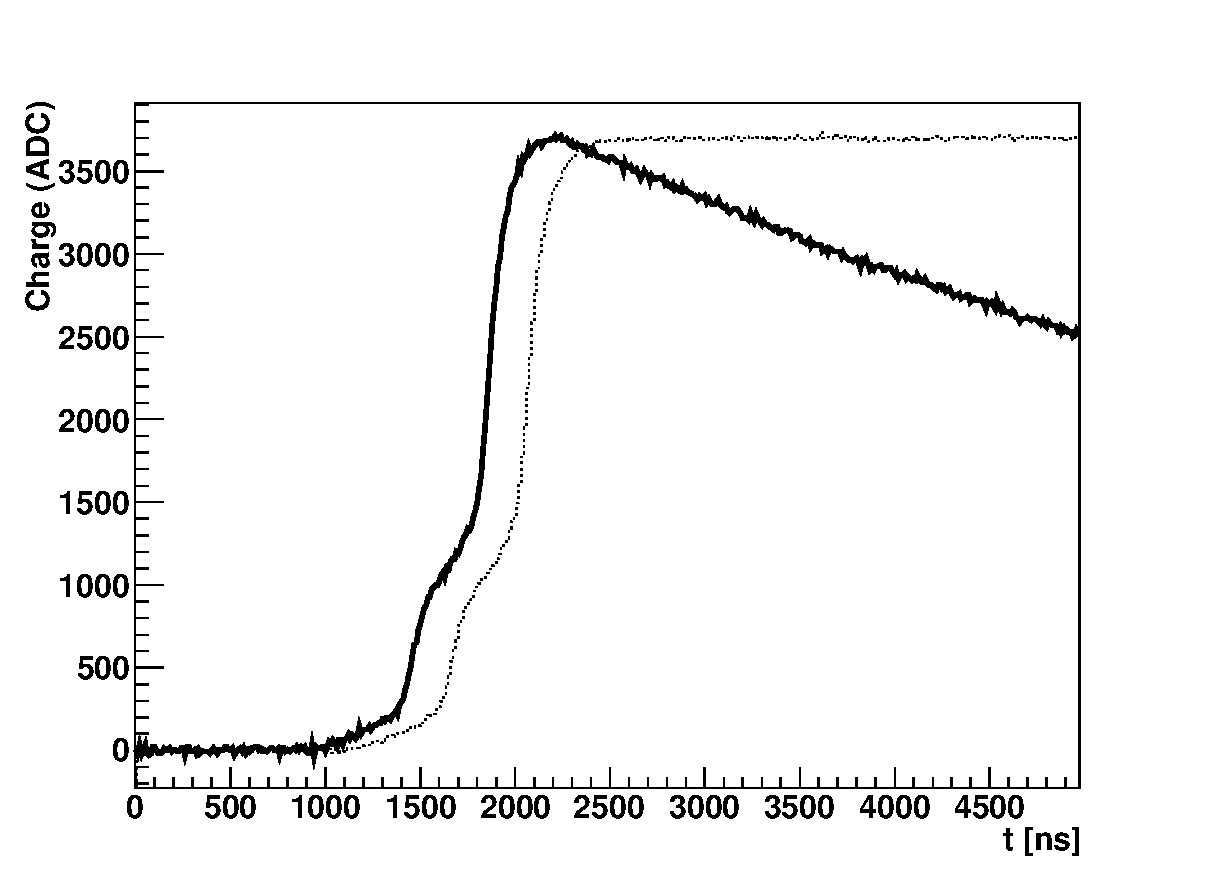
\includegraphics[width=0.9\textwidth]{PPC2WaveformComparison}
				\caption[Visualization of synchronized pulses from the Gretina and Pixie digitizers]
				{Visualization of two synchronized pulses from the Gretina (bold) and Pixie digitizers.  
				The different decay constant are due to the different input impedances of each card.}
				\label{fig:HeadToHeadPulseExample}
			\end{figure}

	 After synchronization, a simple pulse-shape analysis algorithm~\cite{Budjas:2009zu} developed by the GERDA collaboration was applied to the data.  In this algorithm, the ratio $A/E$ is calculated, where $A$ is the maximum of the current pulse (derivative of the charge pulse) and $E$ is the amplitude (energy) of the charge pulse.  This ratio can then be used to discriminate between single- and multi-site events due to the fact that events with multiple interaction sites tend to have wider current pulses for a given energy, $E$.  A version of this algorithm was implemented using waveform processing code in MGDO.  
	 
	 Before processing, the data sets were reduced to include only events in a $\sim$50~keV window around the $^{208}$Tl DEP at 1592.5~keV.  For each event of this subset, the current waveform was generated by using a Savitzky-Golay derivative filter~\cite{Sav64aa} of size~5 and degree~4 and the current maximum was saved.  Cuts were then applied to the data for a range of values for $A/E$ and the data were fit using binned maximum likelihood using the RooFit toolkit~\cite{ver03aa} over the range $1570\to1615$~keV.  This fit was used to estimate the survival probability of the $^{208}$Tl DEP and background reduction in the continuum and nearby peaks, including the 1588.2 and 1580.5~keV gamma peaks of $^{228}$Ac.  An example of such a fit is shown in Figure~\ref{fig:HeadToHeadExampleFit}.  A direct comparison between the pairs of cards is possible by looking at the background reduction and survival probability versus the cut parameter, $A/E$, as calculate for each digitizer.  These results are shown for DGF4-c and Gretina cards in Figure~\ref{fig:HeadToHeadDGF4cResults}, and for the Pixie-4 and Gretina cards in Figure~\ref{fig:HeadToHeadPixie4cResults}.  It is clear from these plots that the 3 cards behave comparably with this particular algorithm.  The only discrepancy exists in the DGF4-c vs.~Gretina results: the DGF4-c has a slightly steeper acceptance curve around an $A/E$ value of 62.
	 
			\begin{figure}
				\centering
				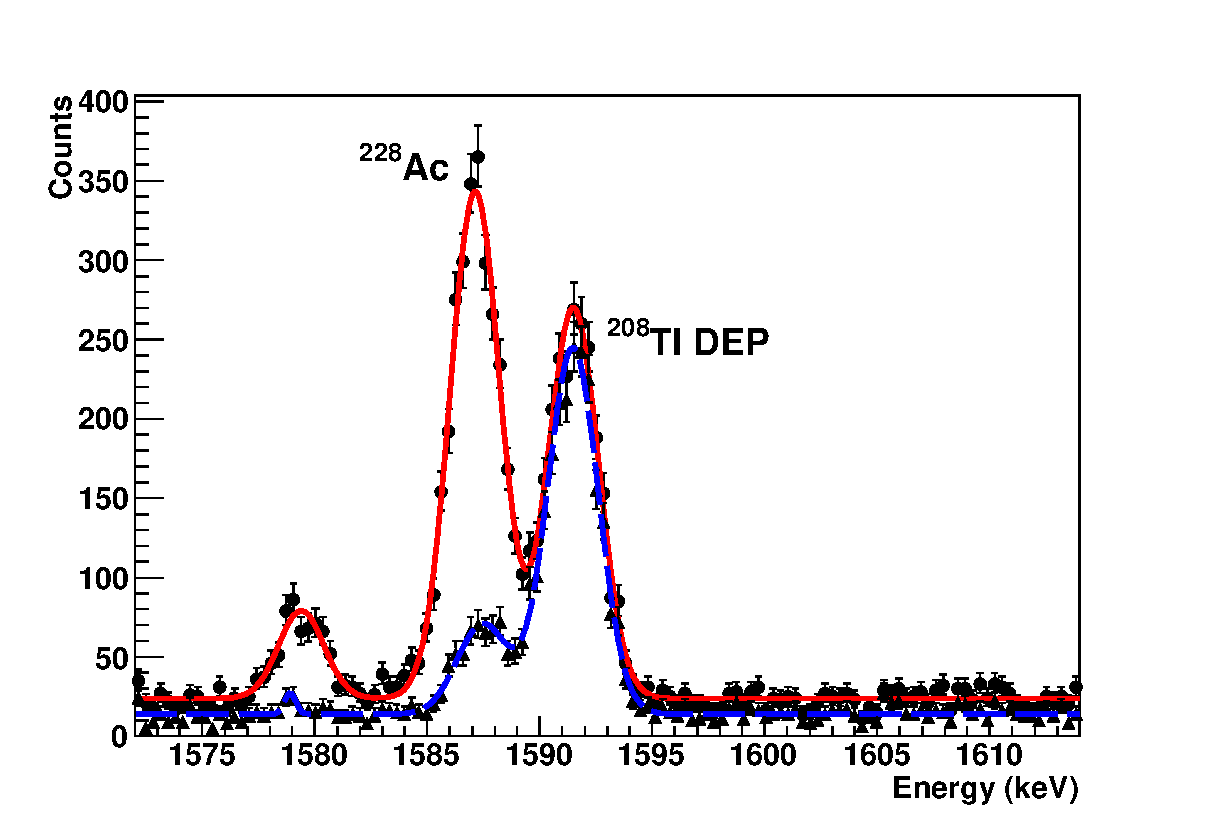
\includegraphics[width=0.9\textwidth]{Tl208DEPFitExample}
				\caption[An example set of fits using the Gretina card]
				{An example set of fits using the Gretina card.  The solid line (circles) is without cuts, the dashed (triangles)
				 with cuts, yielding a signal acceptance of $94.8\pm1.77\%$ in the $^{208}$Tl DEP and a $89.1\pm0.99\%$ 
				 reduction in the adjacent 1588.2~keV $^{228}$Ac peak.}
				\label{fig:HeadToHeadExampleFit}
			\end{figure}	
		
		% Then application of a simple PS analysis.  
			\begin{figure}
				\centering
				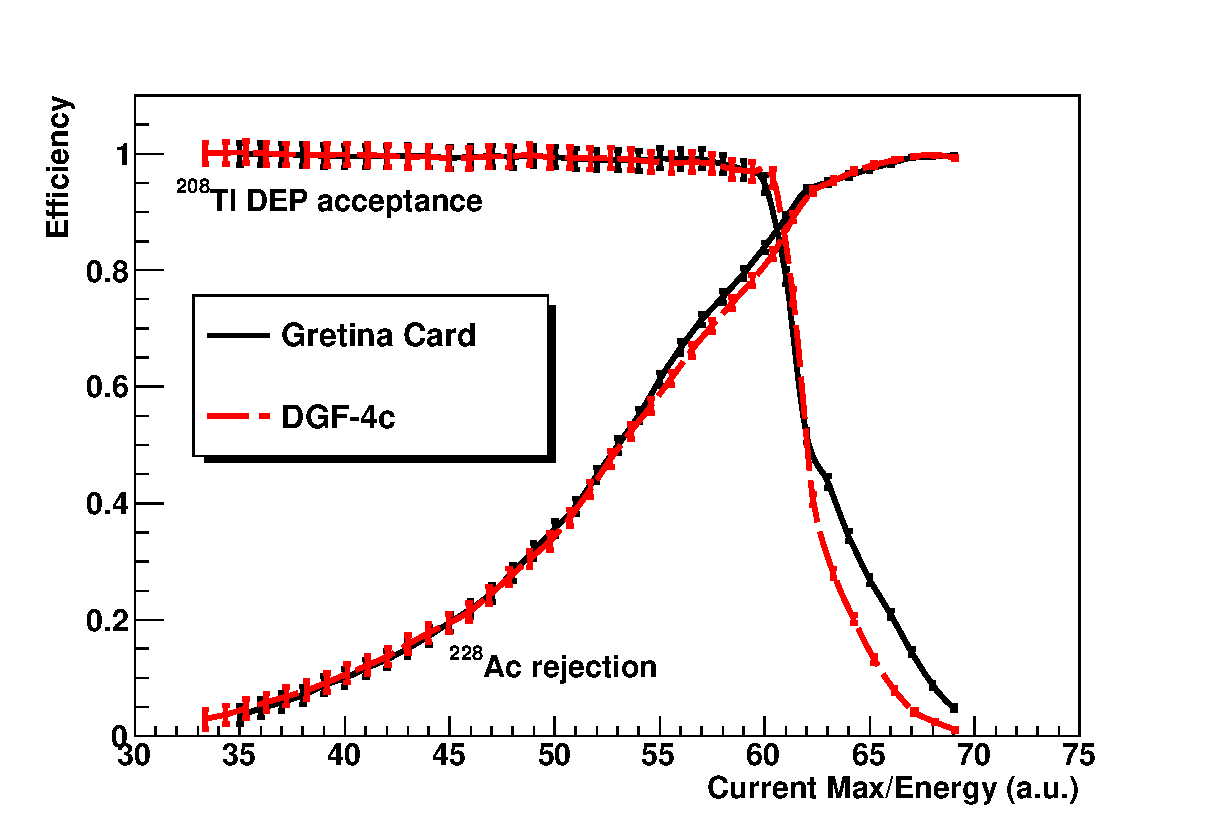
\includegraphics[width=0.9\textwidth]{DGF4c_Vs_Gretina}
				\caption[Cuts for Gretina vs. DGF-4c]
				{Cuts for Gretina vs. DGF-4c.}
				\label{fig:HeadToHeadDGF4cResults}
			\end{figure}	
	
			\begin{figure}
				\centering
				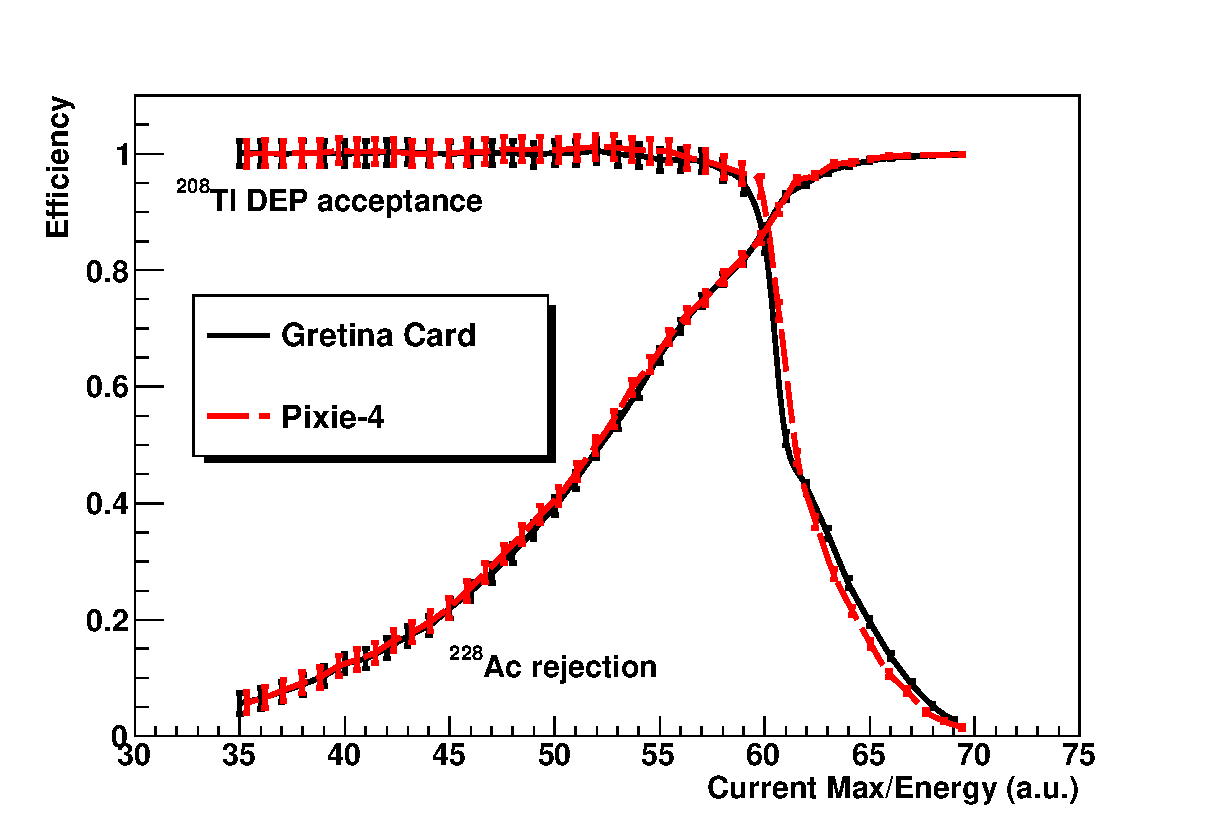
\includegraphics[width=0.9\textwidth]{Pixie_Vs_Gretina}
				\caption[Cuts for Gretina vs. Pixie-4c]{Cuts for Gretina vs. Pixie-4c.}
				\label{fig:HeadToHeadPixie4cResults}
			\end{figure}	
			
		\subsection{Conclusions}
	     	\label{sec:HeadToHeadCompareConclusions}
		
	For the simple pulse-shape algorithm presented here the 3 digitizer cards perform similarly, suggesting that the $A/E$ calculation is not significantly sensitive to the sampling frequency of the fast ADC.  More advanced PSA, such as those based upon comparing pulses to a library of single-site events~\cite{Ren10}, are more likely to depend on the sampling characteristics of the digitizer.  The following sections explore other characteristics of the Gretina digitizer to determine how well its hardware and firmware configuration enable it to perform at low energies.
	
		% Reference Ren's paper, a lot of work that has been done there, understanding that this 
		% is a very simple technique applied to data.     

	\section{Development and testing of the Gretina Mark IV digitizer}
		\subsection{Trigger Design and Tests}
		\label{sec:DeploymentPPC2SoudanTriggerDesign}     
			
	Before deployment of the DAQ system underground in Soudan, triggering tests were performed to determine the optimum conditions for minimizing the energy threshold of the electronics.  The goal of these initial measurements was also to develop an automated set of tests to perform regularly on \ppc2 \emph{in situ}.  Triggering efficiency refers to the probability of inducing a trigger at a particular signal amplitude.  It should be 1 well above threshold and decrease to 0 as the amplitude of the signal reduces below threshold.  The basic technique to measure the trigger efficiency of a detector system is to inject a pulse of known amplitude into the test port of the electronics and complete a series of measurements, adjusting the amplitude of the pulse to sample around the threshold.  One can determine the probability of detecting a pulse by either knowing the rate of the injected pulse and performing the test for a known period of time, or by having an independent measure of the the timing of the injected pulse (i.e.~a synchronization pulse) and performing a coincidence measurement.  For these tests, the latter method was chosen as it was deemed a cleaner technique to extract both the trigger efficiency given a certain pulse amplitude as well as the false trigger rate at a particular threshold setting.  
	
	The test setup included the pulser and computer-controlled attenuators described in Section~\ref{sec:DeploymentPPC2SoudanDAQSystem} and was run by the ORCA DAQ software.  To vary the amplitude of the injected pulse, it was decided to keep the output pulse from the waveform generator constant and change the attenuator settings.  Scripts were designed in ORCA to perform these variations automatically.  The attenuated pulse was amplified using a Phillips 777 before being injected directly into a Gretina card to ensure that the noise of the input signal dominated the intrinsic noise of the digitizer.  The amplitude of the measured pulse was estimated using an offline trapezoidal filter as was done in later analysis (see Section~\ref{sec:DeploymentPPC2SoudanAnalysis}).  Because a similar detector system to \ppc2 was unavailable above ground at the time of the tests, it was impossible to simulate the exact noise environment of \ppc2's electronics.  To circumvent this limitation, all the measurements were determined in terms of signal-to-noise ratios to be able to compare directly to the detector system.  For example, a measured signal-to-noise ratio could be multiplied by the separately measured magnitude of the detector noise to provide a rough calibration of the results.  Manufacturer specifications quoted this value as 180~eV~FWHM\footnote{This value was measured using an analog shaping amplifier and is dependent upon the shaping times of the amplifier.  In practice, this value is different than one calculated using digital shaping (i.e.~with a trapezoidal filter, as was done in this analysis) and so was interpreted as an estimate when compared directly to digital measurements.}~\cite{Orr2007}.  
	
		Initial measurements found that the Gretina on-board trigger, a leading-edge discrimination (LD) differential algorithm with fixed shaping, achieved $\sim$90\% efficiency at an S/N of $\sim$6, suggesting that a similar efficiency would be found at $\sim$1~keV on the detector system.  This was at least a factor of 2 worse performance than demonstrated in analog readout systems with a detector of similar noise characteristics~\cite{Barb07}.  The degraded trigger performance was due to the limited shaping associated with the LD trigger which had not originally been designed to trigger on very-low-amplitude preamp signals.  To solve this issue, a hybrid digital/analog system was designed: the signal was split after the 777, one line running directly to the digitizer and the other into a spectroscopy amplifier with 1~$\mu$s shaping time.  The output from the spectroscopy amplifier was input into the Gretina card and this channel was used to trigger the unshaped input channel.  Longer shaping times were tested, but were found to trigger poorly since the differential algorithm was insensitive to the leading edge of a slower-rising pulse.  Tests with this hybrid system indicated an improvement of triggering efficiency.  Results comparing the two methods are presented in Figure~\ref{fig:PPC2TriggeringEfficiencyTests}.  
	
			\begin{figure}
				\centering
				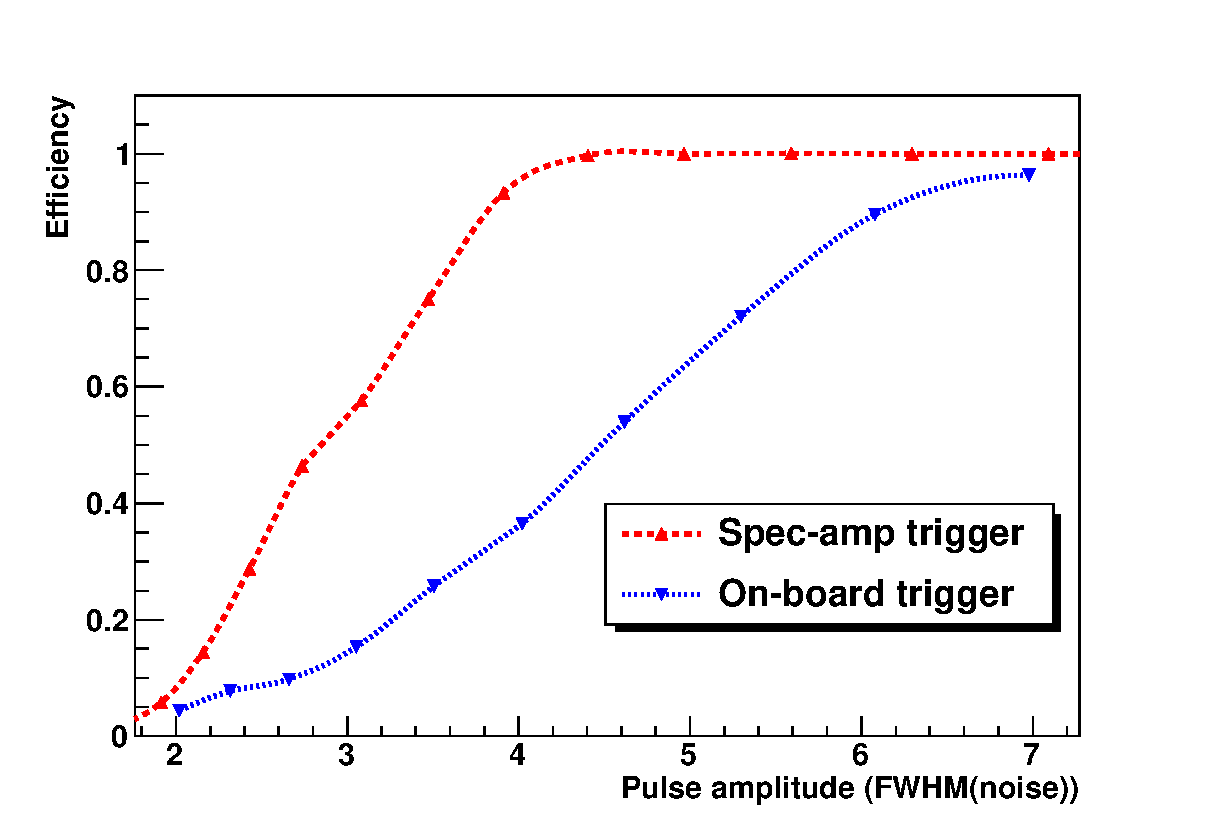
\includegraphics[width=0.9\textwidth]{EfficiencyThreshold}
				\caption[Triggering efficiency test results]
				{Triggering efficiency test results comparing the on-board LD trigger to the 
				hybrid system.  The hybrid system was found to have a factor of $\sim$2 improvement.}
				\label{fig:PPC2TriggeringEfficiencyTests}
			\end{figure}

		\subsection{Measured electronic noise}
		\label{sec:DeploymentPPC2SoudanAnalysisElectronicNoise}    
	
	The electronic noise was measured by injecting a pulse from the waveform generator and calculating the FWHM of the width of the peak.  Since this calculation was performed offline, the parameters of the trapezoidal filter (i.e. integration time and collection time) could be varied over the same data set to determine the values which would yield the best resolution.  The trace length of the waveform was limited to 10~$\mu$s and, since the rising edge of the waveform was positioned in the middle of the digitization window, the offline filter integration length was limited to less than 5~$\mu$s.  In practice, the limitation on the integration time was closer to 3.5~$\mu$s to account for variations in the position of the rising edge of the pulse with different pulse amplitudes.  Results, shown in Figure~\ref{fig:PPC2NoiseVsIntegrationTime}, indicate that the best resolution comes at the longest shaping time and also suggest that the minimum resolution could not be achieved with this setup.  The minimum value measured in this test, 225~eV, was larger than the value measured with an analog electronics system, 180~eV, but it is expected that this difference would shrink if longer integration times were available.
	
				\begin{figure}
					\centering
					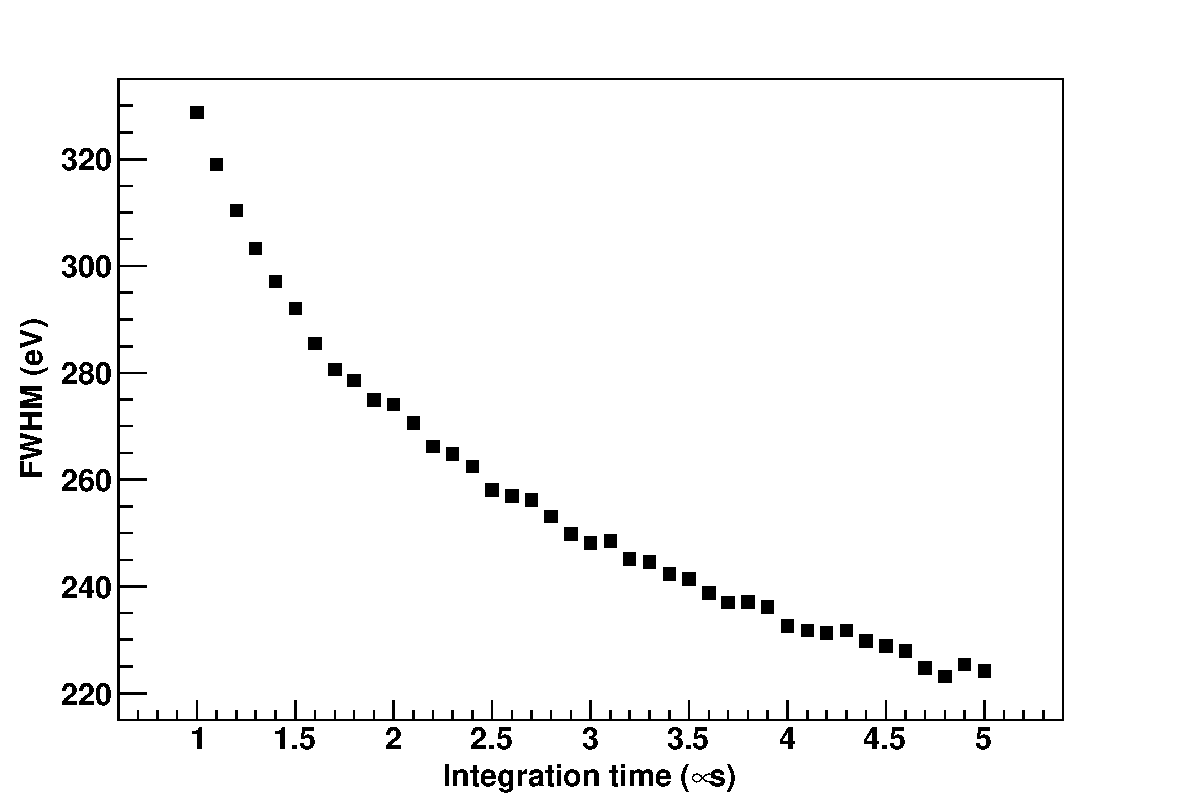
\includegraphics[width=0.9\textwidth]{filterTestTrap1d-1}
					\caption[Noise versus integration time of the trapezoidal filter]
					{Noise versus integration time of the trapezoidal filter.}
					\label{fig:PPC2NoiseVsIntegrationTime}
				\end{figure}
		
		\subsection{Conclusions}
	
	The Gretina card provides sufficient characteristics for physics near the $\nonubb$ Q-value (2~MeV), but does not clearly 
achieve good enough threshold or resolution at low energies in comparison to results from analog systems.  Because of this, additional work beyond the scope of this thesis began, focusing on refining the triggering algorithms and onboard hardware to enable better resolution and triggering capabilities.  This work is focusing on developing these capabilities in two cards, including the Struck 16-bit, 100~MS/s 3302 and the Gretina digitizer.  Despite the low-energy limitations of the tested firmware on the Gretina card, this DAQ system was deployed to readout the \ppc2 detector placed underground at Soudan Underground Laboratory.  Results of this deployment are presented in Chapter~\ref{chap:DeploymentPPC2Soudan}.
%%%%\section{Development of the Struck 3302 Digitizer}
%%%%
%%%%	\subsection{Description of system}
%%%%    
%%%%	\begin{table}
%%%%		\centering
%%%%		\begin{tabular}{l|c|c}
%%%%		\end{tabular}
%%%%		\caption[Differences between the Gretina Digitizer and the Struck Digitizer]
%%%%		{Differences between the Gretina Digitizer and the Struck Digitizer.}
%%%%		\label{tab:BeGeSIS3302GretinaDifferences}
%%%%	\end{table}	
%%%%      
%%%%	\subsection{Analysis and Results}
%%%%	\label{sec:DeploymentBeGeSoudanAnalysis}
%%%%	% Description of analysis techniques used and results.  The ordering of this section could be modified.
%%%%	
%%%%		\subsubsection{Calibration}
%%%%		\label{sec:DeploymentBeGeSoudanAnalysisCalibration}    
%%%%		
%%%%			\begin{figure}
%%%%				\centering
%%%%				%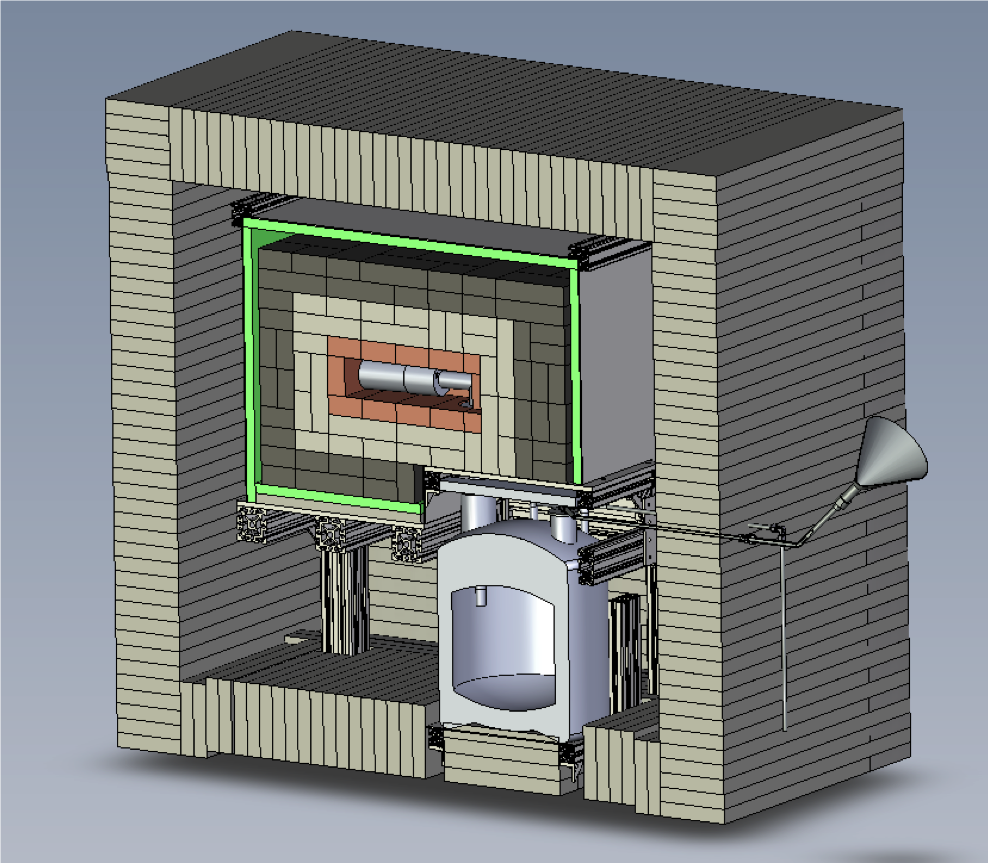
\includegraphics[width=0.9\textwidth]{PPC2DesignSchematicAll}
%%%%				\caption[Calibration of the channels]{Calibration of the channels.}
%%%%				\label{fig:BeGeCalibration}
%%%%			\end{figure}
%%%%	    
%%%%	    	\subsubsection{Trigger Efficiency}
%%%%		\label{sec:DeploymentBeGeSoudanAnalysisTriggerEfficiency}    
%%%%		
%%%%			\begin{figure}
%%%%				\centering
%%%%				%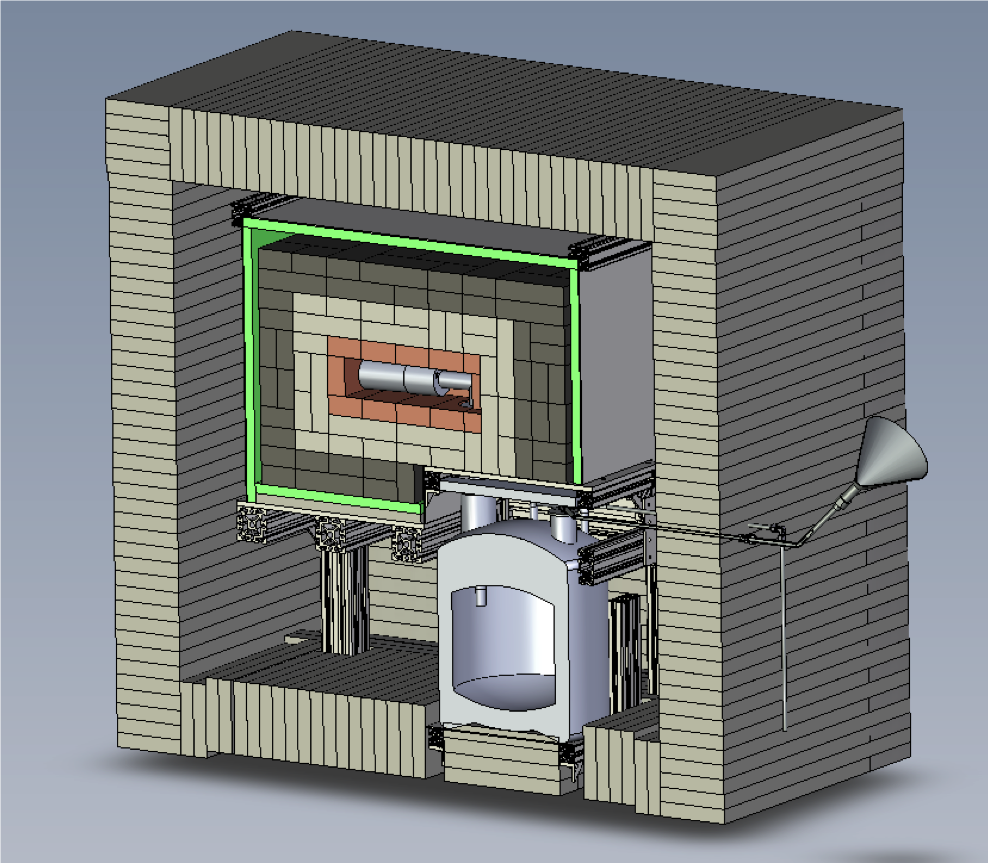
\includegraphics[width=0.9\textwidth]{PPC2DesignSchematicAll}
%%%%				\caption[Struck card triggering efficiency tests]{Triggering efficiency tests.}
%%%%				\label{fig:BeGeTriggeringEfficiencyTestsVsTime}
%%%%			\end{figure}
%%%%		
%%%%	    	\subsubsection{Noise measurement}
%%%%		\label{sec:DeploymentBeGeSoudanAnalysisNoiseMeasurment}    
%%%%		
%%%%			\begin{figure}
%%%%				\centering
%%%%				%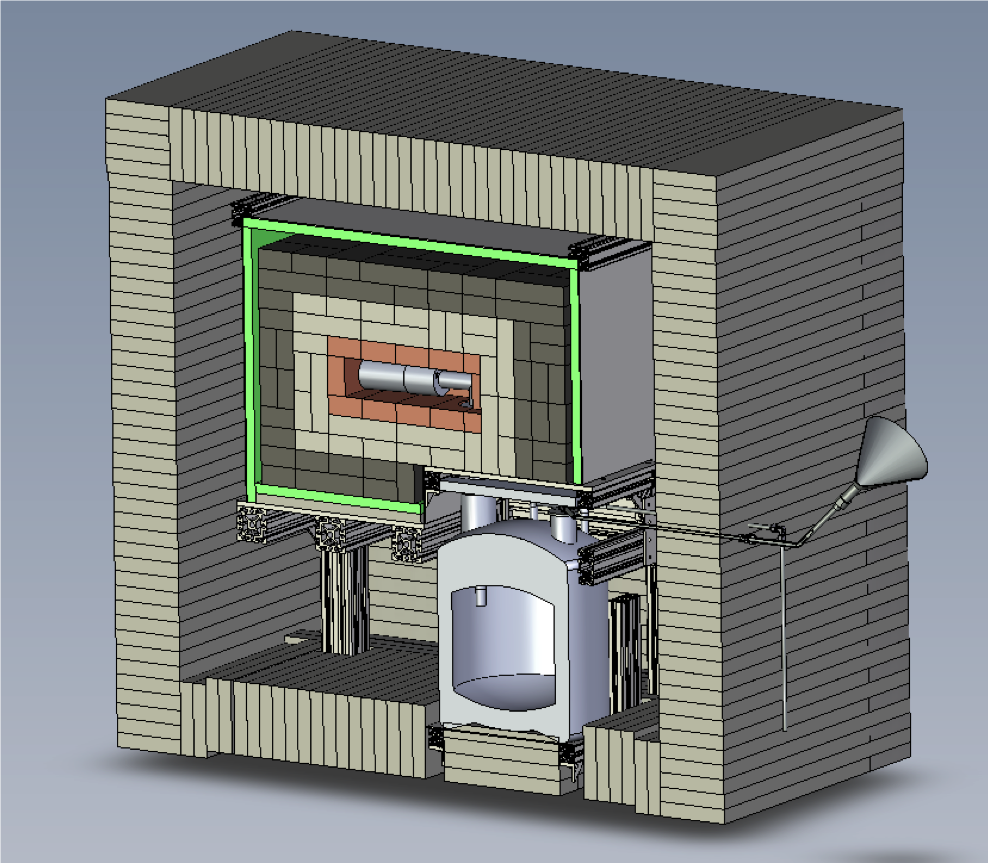
\includegraphics[width=0.9\textwidth]{PPC2DesignSchematicAll}
%%%%				\caption[Struck noise measurement versus integration time]
%%%%				{Noise measurement versus integration time.}
%%%%				\label{fig:BeGeTriggeringNoiseMeasurment}
%%%%			\end{figure}
%%%%					
%%%%	    	\subsubsection{Energy spectra}
%%%%		\label{sec:DeploymentBeGeSoudanAnalysisEnergySpectra}    		
%%%%
%%%%			\begin{figure}
%%%%				\centering
%%%%				%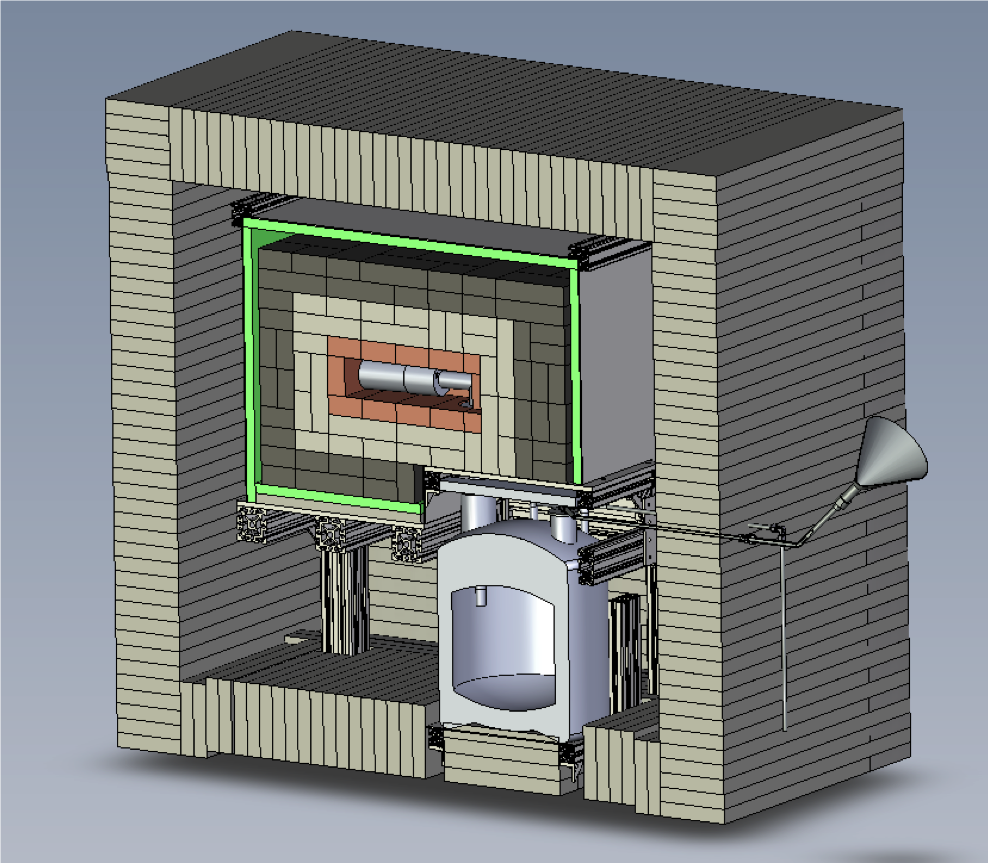
\includegraphics[width=0.9\textwidth]{PPC2DesignSchematicAll}
%%%%				\caption[Struck energy spectrum from high- and low-gain channels]
%%%%				{Energy spectrum from high- and low-gain channels.}
%%%%				\label{fig:BeGeEnergySpectrum}
%%%%			\end{figure}      
%%%%			
%%%%	\subsection{Conclusions}	
%%%%	    




